%! TEX root = ../barycenter.tex
\YYCleverefInput{/var/tmp/latex/barycenter.sed}
\section{Absolute continuity in the general case}

In the general case, we shall apply the consistence of barycenter and
discuss relations between density functions of barycenter measure and marginal measures.
This involves the Jacobian of optimal transport map,
which requires to study the Hessian of $c$-concave functions.
To see it, we introduce the central result of McCann \cite{mccann2001polar} on optimal mass transport,
stated as \cite[Theorem 3.2]{cordero2001riemannian}.
\begin{thm}[Optimal mass transport on manifolds]
	\label{thm:optimal_transport_manifold}
	Let \( M \) be a complete Riemannian manifold.
	Fix two Borel probability measures \( \mu \ll \) $\operatorname{Vol}$ and \( \nu \) on \( M \),
	and two compact subsets \( X \) and \( Y \subset M \) containing the support of \( \mu \) and \( \nu \),
	respectively.
	Then there exists \( \phi \in \mathcal { I } ^ { c } ( X , Y ) \) such that the map
	\begin{equation}
		\label{equa:transform_map}
		T ( x ) : = \exp _ { x } ( - \nabla \phi ( x ) )
	\end{equation}
	pushes \( \mu \) forward to \( \nu \).
	This map is uniquely characterized among all maps pushing \( \mu \) forward \( \nu \) by formula \cref{equa:transform_map} with \( \phi \in \mathcal{I} ^ { c } ( X , Y )\).

	Furthermore, $T$ is the optimal transport map asserted in \Cref{thm:uniquness_monge_problem_manifold}.
\end{thm}

\subsection{Hessian almost everywhere}
The main goal of the following discussion is to define properly the differential
of the optimal mass transport map $T = \exp (- \nabla \phi)$ while even $ \nabla \phi$ only exists almost everywhere.
% In this subsection, we aim to give a proper definition of Hessian
% for $c$-concave function
% though its first order differential is not defined everywhere.
% The following two definitions generalize the concept of gradient;
% and the generalized gradient always exist for $c$-concave functions in contrast to the usual one.
% We shall use it to give a proper definition of Hessian when the usual gradient of
% function is not defined everywhere.
Our first step is generalize the concept of gradient
so that it exists everywhere for $\phi$.
\begin{defn}
	[$c$-super-differential \( \partial ^ { c } \phi \)]
	Let \( X , Y \) be two compact sets of M. For \( \phi \in \mathcal { I } ^ { c } ( X , Y ) \)
	and \( x \in X \), the \( c \)-super-differential of \( \phi \) at \( x \) is the non-empty set
	\begin{align}
		\partial ^ { c } \phi ( x ) : & = \left\{ y \in Y \mid \phi ( x ) + \phi ^ { c } ( y ) = c ( x , y ) \right\}                     \\
		                              & = \{ y \in Y \mid \phi ( z ) \leq \phi ( x ) + c ( z , y ) - c ( x , y ), \quad \forall z \in X \}
		\label{equa:c-super-differential}
	\end{align}
\end{defn}

\begin{example} [Multivalued extension]
	\label{example:minimizer_differentiable}
	According to \Cref{lem:minimizer_differentiable},
	if \( \phi \in \mathcal { I } ^ { c } ( \widebar {\mathcal{X} } , Y ) \) is differentiable at
	\( x \in \mathcal { X } \subset \subset M \),
	then \( \partial ^ { c } \phi ( x ) = \{ F ( x ) \} = \left\{ \exp _ { x } ( - \nabla \phi ( x ) ) \right\} \).
\end{example}

\begin{defn}[Super-gradient and super-differential]
	A function \( \phi : \Omega \rightarrow \mathbb { R } \) defined on an open subset \( \Omega \) of \( M \)
	is said to be super-differentiable at \( x \in \Omega \) with super-gradient \( v \in T _ { x } M \) if for
	\( u \rightarrow 0 \in T _ { x } M \),
	\begin{equation}
		\label{equa:super-differential}
		\phi \left( \exp _ { x } u \right) \leq \phi ( x ) + \langle v , u \rangle + o ( | u | ).
	\end{equation}
	The super-differential of \( \phi \) at \( x \) refers to
	the convex set \( \partial \phi ( x ) \subset T _ { x } M \) of all super-gradients at \( x \).
\end{defn}

% One can easily check that a function is differentiable if it is both
% super-differentiable and sub-differentiable.
A typical example of a function which admits super-gradients everywhere
is the square distance \( d _ { y } ^ { 2 } / 2 \) to \( y \in M \).
Indeed, if \( \gamma \) is a minimal geodesic
joining \( x = \gamma ( 0 ) \) to \( y = \gamma ( 1 ) \),
then \( - \dot { \gamma } ( 0 ) \in \partial \left( d _ { y } ^ { 2 } / 2 \right) ( x ) \)  as shown in \cite[Proposition 7]{mccann2001polar}.
The following lemma \cite[Lemma 3.7]{cordero2001riemannian} claims that
this is a general property of $c$-concave functions.

\begin{lem}[$c$-super-gradients imply super-gradients]
	\label{lem:c-super-gradients_imply_super-gradients}
	Fix \( \mathcal { X } \subset \subset M \) open,
	\( Y \subset M \) compact, and \( \phi \in \mathcal { I } ^ { c } ( \widebar { \mathcal{X} } , Y ) \).
	Let \( ( x , y ) \in \mathcal { X } \times Y \) and \( v \in T _ { x } M \) satisfy
	\( | v | = d ( x , y ) \) and \( \exp _ { x } ( - v ) = y\).
	If \( y \in \partial ^ { c } \phi ( x ) \) then
	\( v \in \partial \phi ( x ) \).
\end{lem}
Hence, a $c$-concave function has always super-differential.
Our definition of Hessian is based on super-differential.

\begin{defn}[Hessian]
	Let \( \phi : \Omega \rightarrow \mathbb { R } \) be a	super-differentiable function on an open set \( \Omega \subset M \).
	We say that \( \phi \) has \( a \) Hessian \( \operatorname{Hess}_x\phi \) at \( x \in \Omega \) if \( \phi \) is differentiable at \( x \)
	and there exists a self-adjoint operator \( \operatorname{Hess}_x \phi : T _ { x } M \rightarrow T _ { x } M \) satisfying
	\begin{equation}
		\label{defn:hessian}
		\sup _ { v \in \partial \phi \left( \exp _ { x } u \right) }
		\left| \Pi _ { x , u } v - \nabla \phi ( x ) - \operatorname{Hess}_x \phi (u) \right| = o ( | u | )
	\end{equation}
	as \( u \rightarrow 0 \) in \( T _ { x } M \).
	Here \( \Pi _ { x , u } : T _ { \exp _ { x } u } M \rightarrow T _ { x } M \) denotes the parallel translation to \( x \) along the geodesic \( \gamma ( t ) : = \exp _ { x } \left( (1-t) u  \right)\), $t \in [0,1]$.
\end{defn}

This definition coincides with the usual one for smooth functions.
A more intuitive understanding of the Hessian follows from the fact that
existence of a Hessian \( \operatorname{Hess}_x \phi \) at \( x \) for \( \phi \) implies a second order Taylor expansion for \( \phi \) around \( x : \) as \( u \rightarrow 0 \in T _ { x } M \),
\begin{equation}
	\label{equa:hessian_expan}
	\phi \left( \exp _ { x } u \right) = \phi ( x ) + \langle \nabla \phi ( x ) , u \rangle +
	\frac { 1 } { 2 } \langle \operatorname{Hess}_x \phi (u) , u \rangle + o \left( | u | ^ { 2 } \right).
\end{equation}

The following theorem (see \cite[Proposition 3.4]{cordero2001riemannian}) justifies the usage of the word ``concave''.
\begin{thm}[$c$-concave function admits a Hessian almost everywhere]
	\label{thm:c-concave_hessain}
	Let $\mathcal{X} \subset \subset M$ be open and $Y \subset M$ be compact.
	Every $c$-concave function in $\mathcal{I}^c(\widebar { \mathcal{X}}, Y )$ admits a Hessian
	almost everywhere with respect to the volume measure on $M$.
\end{thm}

\begin{prop} [Differentiating optimal transport]
	\label{prop:differentiate_optimal_transport}
	Fix an open set \( \mathcal{X} \subset \subset M \) and a compact set \( Y \subset M \).
	Let \( \phi \in \mathcal{I} ^ { c } ( \widebar { \mathcal{X} } , Y ) \) and set \( F ( z ) : = \exp _ { z } ( - \nabla \phi ( z ) ) . \)
	Fix a point \( x \in \mathcal{X} \) where \( \phi \) admits a Hessian in the sense of \cref{defn:hessian}.
	\begin{enumerate}
		\item Define \( y : = F ( x ) \notin \operatorname { cut } ( x ) \) and \( H : = \operatorname { Hess } _ { x } d _ { y } ^ { 2 } / 2 \), then we have \( H - \operatorname { Hess } _ { x } \phi \) \( \geq 0 \).
		\item Define \( Y : = \diff \left( \exp _ { x } \right) _ { - \nabla \phi ( x ) } \) and
			\( \diff F _ { x } : = Y \left( H - \operatorname { Hess } _ { x } \phi \right)\)
			from $T_x M$ to $T_y M$.
		      Then as \( u \rightarrow 0 \) in \( T _ { x } M \),
		      \begin{equation}
			      \label{equa:differentiate_optimal_transport}
			      \sup _ {\substack {\exp _ { y } v \in \partial ^ { c } \phi \left( \exp _ { x } u \right) \\
					      | v | = d \left( y , \exp _ { y } v \right)} } \left| v - \diff F _ { x } ( u ) \right| = o ( | u | ).
		      \end{equation}

	\end{enumerate}
\end{prop}

It helps to mention that by \Cref{example:minimizer_differentiable} we have
$\partial^c \phi (x) = \{ F(x) \}$.
Then the cryptic \cref{equa:differentiate_optimal_transport} means that we are differentiating
the set valued map $z \mapsto \partial^c \phi(z)$.
As $c$-super-differential gives rise to a super-differential by \Cref{lem:c-super-gradients_imply_super-gradients},
it makes sense to compare the differential $\diff F_x$ with all super-differentials $v$.
\begin{rmk}[Sketch proof for the second point of \Cref{prop:differentiate_optimal_transport}]
	% For the first point, we apply the characterization of cut locus in \Cref{prop:distance_cut_locus};
	% existence of Hessian for $\phi$ and \cref{equa:c-concave_conjugate} then gives a lower bound for squared distance function $d_y^2$.

	% 	As for the second point,
	It is a clever application of chain rule and \cref{equa:exponential_map_and_squared_distance_function}.
	Ignore the problem of second differentiability for a while, we define
	\[
		g(u,v) = \exp_{u}(-\nabla d_y^2(u) + \nabla d_y^2(v) - \nabla \phi (v)),
	\]
	then $F(z) = g(z, z)$ and $ y = g(u, x) $ is a constant $y := F(x)$.
	This gives that
	\[
		\diff F(x) = \partial_u g(x, x) + \partial_v g(x, x) = \partial_v g(x, x) = Y(H - \operatorname{Hess}_x \phi).
	\]
	For a full proof, see \cite[Proposition 4.1]{cordero2001riemannian}.
\end{rmk}

This definition of differential gives Jacobian identity \cite[Theorem 4.2]{cordero2001riemannian}.

\begin{thm}
	[Jacobian identity a.e.]
	\label{thm:jacobian_identity}
	Let \( \mu \ll \operatorname{Vol} \) and \( \nu \ll \operatorname{Vol} \) be
	two compactly supported Borel probability measures and denote their
	\( L ^ { 1 } ( M, \operatorname{Vol}) \) densities by \( f \) and \( g \), respectively.
	Fix domains \( \mathcal{X} \subset \subset M \) and \( \mathcal{Y} \subset \subset M \) containing the support of \( \mu \) and \( v \), respectively.
	Suppose that \( \phi \in \mathcal{I} ^ { c } ( \widebar { \mathcal{X} } , \widebar { \mathcal{Y} } ) \) induces
	\( F : \mathcal{X} \rightarrow \widebar { \mathcal{Y} } \) defined by \( F ( x ) : = \exp _ { x } ( - \nabla \phi ( x ) ) \)
	which pushes \( \mu \) forward to $\nu$.
	Then there exists a Borel set \( K \subset \mathcal{X} \) of full
	measure for \( \mu \) such that
	\begin{enumerate}
		\item $\phi$ admits a Hessian \( \operatorname { Hess } _ { x } \phi \) at each \( x \in K \), and hence \( F ( x ) \notin \operatorname { cut } ( x ) \);
		\item for \( x \in K \), setting \( Y : = \diff \left( \exp _ { x } \right) _ { - \nabla \phi ( x ) } \) and \( H : = \operatorname { Hess } _ { x } d _ { F ( x ) } ^ { 2 } / 2 \), one
		      has
		      \[ f ( x ) = g ( F ( x ) ) \operatorname { det } \left[ Y \left( H - \operatorname { Hess } _ { x } \phi \right) \right] \neq 0 .\]
	\end{enumerate}
\end{thm}

We remark that in the proof of this theorem,
it is shown (see \cite[Claim 4.3 and Claim 4.4]{cordero2001riemannian}) that
$\det \diff F_x > 0$ holds $\mu$ almost everywhere.
% And in general $ \det \diff F_x \geq 0$ holds (\cite[Lemma 2.1]{cordero2001riemannian})
% whenever it exists.

\subsection{Jacobian Bound and sectional curvature}

Using sectional curvature, we can bound $Y$ and $H$ in the expression $\det[ Y(H - \operatorname{Hess}_x \phi)]$.
For $\operatorname{Hess}_x \varphi$, as we shall see
in the proofs of \Cref{thm:absolute_continuity_discrete} and \Cref{thm:absolute_continuity_general},
either
\begin{itemize}
	\item $\phi = g_1$ is a linear combination of squared distance functions and we can apply the bound for $H$,
	\item either we remove several $\operatorname{Hess}_x\phi$ at the same time using minimality of barycenter.
\end{itemize}
% We bound them using Ricci curvature and
% we can prove these bounds using similar compassion arguments involving Jacobi field.
% We define
% \begin{equation}
% 	S _ { K } ( d ) = \left\{
% 	\begin{array} { l l } \frac { \sin ( \sqrt { K } d ) } { \sqrt { K } d } & \text { if } K > 0 \\
%               1                                                          & \text { if } K = 0
%               \\ \frac { \sinh ( \sqrt { - K } d ) } { \sqrt { - K } d } & \text { if } K < 0
% 	\end{array} \right.
% \end{equation}

Rauch theorem gives bound on $Y$ through section curvature, see
\cite[Theorem IX.2.3]{chavel2006riemannian} for a proof using Jacobi field.
\begin{prop} [The geometric Rauch theorem]
	Let $\xi$ be unit tangent vector in $T_x M$
	and $\gamma$ a geodesic starting at $x \in M$ with initial speed tangent vector $\xi$.
	Suppose \( - k < 0 \) is a lower bound for
	the sectional curvatures at every point of \( \gamma \).
	Assume that \( y = \gamma (t)\) is not in the cut locus of $x$.
	% has no points conjugate to \( p \) along \( \gamma \mid_{( 0 , t ]} \).
	Then, for all \( v \in \xi ^ { \perp } \),
	\begin{equation*}
		% \frac { \mathbf { S } _ { \delta } ( t ) } { t } \leq
		\frac { \left| \diff ( \exp _ { x })  _ {t \xi } \,
			\mathfrak{J}_{t \xi}( v )\right| } { | v | }
		\leq \frac { \sinh (\sqrt{ -k } t )} {\sqrt{-k} t },
	\end{equation*}
	where $\mathfrak{J}_{t \xi}: T_x M \rightarrow T_{t \xi} T_x M$ is the canonical identification
	between these two tangent spaces.
	Note that on the right hand side, $t = d(x,y)$ is the distance between $x$ and $ y = \gamma(t) = \exp_x (t\xi)$.
\end{prop}

The following bound (\cite[Lemma 3.12]{cordero2001riemannian}) on $H$ is proved using a similar argument.
\begin{prop}[Hessian bound for distance squared]
	\label{lem:hessian_bound_distance_squared}
	Fix \(  x , y \in M \) and
	a minimal geodesic \( \gamma \) joining \( x \) to \( y \).
	Suppose \( - k < 0 \) is a lower bound for
	the sectional curvatures at every point of \( \gamma \).
	Each \( u \in T _ { x } M \) satisfies
	\begin{equation*}
		\label{equa:hessian_bound_distance_squared}
		\limsup _ { r \rightarrow 0 } \frac { d _ { y } ^ { 2 } \left( \exp _ { x } r u \right) + d _ { y } ^ { 2 } \left( \exp _ { x } - r u \right) - 2 d _ { y } ^ { 2 } ( x ) }
		{ r ^ { 2 } } \leq 2 \frac{ \sqrt { k } d ( x , y ) }
		{\tanh ( \sqrt { k } d ( x , y ) )}
	\end{equation*}
\end{prop}
% As observed in \cite[Lemma 2.7]{KIM2017640}, with the same proof as \cite[Lemma 3.12]{cordero2001riemannian},
% we can concatenate sectional curvature to get conclusion in Ricci curvature.
% \begin{lem}
% 	Suppose \( - K \leq 0 \) is a lower bound for the Ricci curvature on \( M \).
% 	Then
% 	\[
% 		\operatorname { tr } \left[ \operatorname{Hess}_x d^ { 2 }_y ( x ) \right]
% 		\leq n \frac { \sqrt { K } d ( x , y ) }
% 		{ \tanh ( \sqrt { K } d ( x , y ) ) } .
% 	\]
% \end{lem}

\begin{rmk}
	\label{rmk:global_hessian_bound}
	The right-hand sides of these two bounds are not bounded functions,
	thus we must prove a priori bounds on the distance and section curvature.
	We do this by imposing to the geodesic endpoints to lie in compact sets.

	To be precise, let $X$ and $Y$ be two compact subsets of $M$.
	Every \( x \in X \) and \( y \in Y \) is linked by a minimal geodesic since the manifold \( M \) is complete.
	For our appliaction later, it is safe to assume that $x$ is not in the cut locus of $y$.
	The union \( U \) of all such minimal geodesic segments
	starting in \( X \) and ending in \( Y \) is a closed bounded set, by compactness of \( X \) and \( Y \).
	Also the distances appeared on the right hand sides are bounded from above.
	Therefore,
	if $x$ and $y$ are a priori in two compact sets and $x$ is not the cut locus of $y$,
	then bounds on the right hand sides in these two proposition can be replaced by a global constant
	for these $x$ and $y$.
\end{rmk}

\subsection{Absolute continuity of barycenter by consistency}

\begin{thm}[Absolute continuity of the barycenter of $\sum_{i=1}^n \lambda_i \delta_{\mu_i}$]
	\label{thm:absolute_continuity_discrete}
	Let $M$ be a complete Riemannian manifold.
	Let $\mu_i \in \mathcal{W}_2(M), 1 \leq i \leq n $ be $n$ measures on $M$ with compact supports.
	Assume at least one of them is absolutely continuous
	(with respect to the volume measure on $M$),
	then the unique barycenter $\widebar{\mu}$ of $\sum_{i=1}^n \lambda_i \delta_{\mu_i}$ is also absolutely continuous
	with compact support.
\end{thm}

\begin{proof}

	For simplicity we assume that $\mu_1$ is absolutely continuous.
	Using \Cref{thm:topology_Wasserstein}, we
	approximate $\mu_i, 2 \leq i \leq n $ in $(\mathcal{W}_2(M), W_2)$ by
	a sequence of discrete measures $\{\mu_i^{m}\}_{m \in \mathbb{N}}, 2 \leq i \leq n$,
	concentrated in the compact support of $\mu_i$,
	then $\mathbb{P}_m := \lambda_1 \delta_{\mu_1} + \sum_{i = 2}^n \lambda_i \delta_{\mu_i^m}$ converges to $\mathbb{P}$
	in $\mathcal{W}_2(\mathcal{W}_2(M))$.
	By the consistency of barycenter in the Wasserstein space $\mathcal{W}_2(M)$, i.e.,
	\Cref{thm:consistency_barycenter_Wasserstein},
	the unique barycenter $\widebar{\mu}_m$ of $\mathbb{P}_m$
	converges in $(\mathcal{W}_2(M), W_2)$ to the unique barycenter $\widebar{\mu}$ of $\mathbb{P}$.
	We already show that $\widebar{\mu}_m$ are absolutely continuous in \Cref{section:discrete_measures}.
	Note that $\bar{\mu}$ has compact support by \Cref{rmk:barycenter_compact}.

	We shall show that
	for any $\epsilon > 0$ there is a $\delta > 0$ and $C >0 $ such that for all $m$ we have
	\begin{equation}
		\label{equa:absolutely_continous}
		\forall E \subset M \, \text{measurable, } \operatorname{Vol}(E) < \delta / C^n
		\implies \widebar{\mu}_m(E) < \epsilon.
	\end{equation}
	From \Cref{rmk:global_Lipschitz_constant},
	$C$ should be a global Lipschitz constant for $\exp(-\nabla g_1)$
	in the compact support of $\bar{\mu}$ when $x_i$ varies in the compact support of $\mu_i^m$;
	recall that we define $g_1(x):= - \frac{1}{\lambda_1} \sum_{i=2}^n \lambda_i d(x, x_i)^2$.
	We have $\diff \exp(-\nabla g_1) = Y ( H - \operatorname{Hess}g_1)$
	and $H-\operatorname{Hess} g_1 \geq 0$
	by \Cref{prop:differentiate_optimal_transport};
	moreover, $Y$ is bounded by \Cref{rmk:global_hessian_bound}.
	Note that
	\[
		H-\operatorname{Hess}_x g_1=
		\operatorname{Hess}_xd^2_y + \frac{1}{\lambda_1} \sum_{i=2}^n \lambda_i \operatorname{Hess}_x d^2_{x_i}
		\quad \text{where }y=\exp_x( -\nabla g_1(x))
	\]
	is also bounded from above by \Cref{rmk:global_hessian_bound}.
	Therefore, the Lipschitz constant $C$ we claimed exists.
	% In our situation, a uniform $\delta$ can be chosen for all $\widebar{\mu}_m$
	% because a global Lipschitz constant (independent of $m$)
	% of $\exp( - \nabla g_1)$ exists on the compact set of all possible barycenters.
	% Note that $\widebar{\mu}$ is concentrated on this compact set.
	% $\widebar{\mu}_m$ is pushed by $T_1^{m}$ from $\mu_1$ with a Lipschitz constant bound
	% independent of $m$.

	Recall that for an open set $E \subset M$, $\widebar{\mu}(E) \leq \liminf \widebar{\mu}_m(E)$.
	So
	% because indicator function of open set is lower semi-continuous.
	% Hence, \cref{equa:absolutely_continous} holds for all open sets.
	$\operatorname{Vol}(E) < \delta / C^n \implies \widebar{\mu}(E) < \epsilon$
	by \cref{equa:absolutely_continous}.
	As the Borel measure $\bar{\mu}$ is outer regular, for general measurable $E$ with
	$\operatorname{Vol}(E) < \delta / (2C^n)$,
	we can find an open set $E^\prime$ such that
	$ E \subset E^\prime$ and $ \operatorname{Vol}(E^\prime) < \delta$.
	It follows that $\widebar{\mu}(E) \leq \widebar{\mu}(E^\prime) < \epsilon$
	and $\bar{\mu}$ is absolutely continuous.
\end{proof}

We continue our discussion in the context of this \Cref{thm:absolute_continuity_discrete}.
Let $T_i:=\exp(-\nabla u_i)$ be the optimal transport map from $\widebar{\mu}$ to $\mu_i$,
where $u_i \in \mathcal{I}^c(\widebar{\mathcal{X}}, \overline{\mathcal{Y}_i})$ is a $c$-concave function
and $\mathcal{X}, \mathcal{Y}_i \subset \subset M$ are open sets that contain supports of
$\bar{\mu}$ and $\mu_i$ respectively.

We want first to remove the Hessian of $u_i$ through
the following discussion since it is not well understood.
Let $B(x_1,\ldots,x_n)$ be a measurable selection of barycenter of $\sum_{j=1}^n \lambda_j \delta_{x_j}$.
By the uniqueness of optimal transport map from $\widebar{\mu}$ to $\widebar{\mu}$,
we have $B(T_1, \ldots, T_n) = \operatorname{Id}$ for $\widebar{\mu}$ almost everywhere on $\widebar{\mathcal{X}}$.
Let $\Omega \subset \mathcal{X} $ be a measurable set with $\widebar{\mu}(\Omega) = 1 $ such that
this identity holds and each $\nabla u_i$ admits a Hessian.
We have, for $z \in \Omega$, $B(T_1(z), \ldots, T_n(z))=z$;
it implies that $z$ is the unique barycenter of
measure $\sum_{i=1}^n \lambda_i \delta_{T_i(z)}$ on $M$ and
\[
	W_2(\sum_{i=1}^n \lambda_i \delta_{T_i(z)}, M) \leq \sum_{i=1}^n \lambda_i d_{T_i(z)}^2(x),\quad \forall x \in M
\] with equality at $x=z$.
As $z$ is not in the cut locus of any $T_i(z)$,
we can differentiate twice this inequality at $z \in M$
and then use minimality at $z$ to get
\[
	\sum_{i=1}^n \lambda_i \diff d^2_{T_i(z)} (z) =\sum_{i=1}^n 2 \lambda_i \nabla u_i (z) =0
	,\quad \sum_{i=1}^n \lambda_i \operatorname{Hess}_z u_i \geq 0,
\]
where we use $\nabla u_i(z) = \nabla d^2_{T_i(z)}(z)/2$ by the second point of \Cref{lem:minimizer_differentiable}.
On the other hand, from the definition of $\diff T_i$ in \Cref{prop:differentiate_optimal_transport},
we write $\diff T_i = Y_i ( H_i - \operatorname{Hess}_z u_i)$;
recall that $Y_i := \diff (\exp_z)_{-\nabla u_i}$
and $H_i := \operatorname{Hess}_z d^2_{T_i(z)}$.
As shown in \cite[Lemma 2.1]{cordero2001riemannian}, $\det Y_i >0$,
so $Y_i^{-1} \diff T_i = H_i - \operatorname{Hess}_z u_i \geq 0$.
We can then apply Minkowski's
inequality for determinants of non-negative matrices twice,
\begin{equation}
	\label{equa:remove_hessian_u_i}
	\sum_{i=1}^{n} \det[ \lambda_i Y_i^{-1} \diff T_i]^{1/m}
	\leq
	\det [\sum_{i=1}^n \lambda_i(H_i - \operatorname{Hess}_z u_i)]^{1/m}
	\leq
	\det [\sum_{i=1}^n \lambda_i H_i]^{1/m},
\end{equation}
where $m := \dim M$ is the dimension of $M$
and we use $\sum_{i=1}^n \lambda_i H_i \geq \sum_{i=1}^n \lambda_i \operatorname{Hess}_z u_i \geq 0$.
Note that we manage to remove $\operatorname{Hess}_z u_i$
in \cref{equa:remove_hessian_u_i}.

To ease our notation, we consider the case when $\mu_j, 1 \leq j \leq k$
for some $k \leq n$ are absolutely continuous.
Denote by $\widebar{h}$ the density of $\widebar{\mu}$ and
by $h_j$ the density of $\mu_j$.
Up to removing a $\widebar{\mu}$ measure zero subset of $\Omega$,
we can assume that $\det [\diff T_j] >0$ and
the Jacobian identity in \Cref{thm:jacobian_identity}, i.e.,
$\widebar{h} = h_j \circ T_j \det [\diff T_j]$,
holds on $\Omega$ for $ 1\leq j \leq k$.

We denote by $v_H$ and $v_Y$ the supremums of absolute value
of eigenvalues of $\sum_{i=1}^n \lambda_i H_i$ and $Y_j, 1 \leq j \leq k$
(in a global choice of normal coordinate system on $M$)
respectively at $z \in \Omega$;
they depend on $z$.
% from previous discussion, these two positive numbers only depend on $\mathcal{X}$ and all $\mathcal{Y}_j$.
% In a more precise sense, they depend on lower bound of sectional curvature on $M$
% and maximal distance that all $T_j$ could push.
Apply these bounds at $z \in \Omega$, we get
\begin{equation}
	\label{equa:bound_v_H}
	\sum_{j=1}^k (\lambda_j / v_Y) \det [ \diff T_j]^{1/m} \leq
	\det[\sum_{j=1}^k \lambda_j (H_j - \operatorname{Hess}_z u_j)]^{1/m}\leq
	\det [\sum_{i=1}^n \lambda_i H_i]^{1/m}
	% - \det [\sum_{i>j}^n \lambda_i(H_i - \operatorname{Hess}_z u_i)]^{1/m}
	% - \det [\sum_{i=1}^n \lambda_i \operatorname{Hess}_z u_i]^{1/m}
	\leq v_H
\end{equation}
% Put them into the inequality for $\det [\diff T_i] \geq 0$,
% for $\widebar{\mu}$ almost everywhere,
\textcolor{red}{Here the bad thing is that $v_H$ \textbf{depends on all} $H_i$ for $ 1 \leq i \leq n$
instead of only for $1 \leq i \leq k$}.
Therefore, by the Jacobian identity $\widebar{h} = h_j \circ T_j \det [\diff T_j]$,
\begin{equation}
	\label{equa:density_inequality}
	\widebar{h} \leq (v_H v_Y)^m \left[  \sum_{j=1}^k \frac{ \lambda_j }
		{ (h_j \circ T_j)^{1/m}} \right]^{-m}
	\leq \frac{ (v_H v_Y)^m }{(\sum_{j=1}^k \lambda_j)^{m+1}}
	\sum_{j=1}^k \lambda_j h_j \circ T_j
\end{equation}
where we use Jensen inequality for convex function $x \mapsto x^{-m}$
with linear combination coefficients $\lambda_j / \sum_{j=1}^k \lambda_j$.
% If $g_j$ are bounded by a positive real $l>0$ and
% have supports in a common compact set $K \subset M$.
% Then $\widebar{\mu}(E) \leq (v_H v_Y)^m l \operatorname{Vol}(E)$.

For a compact set $K \subset M$ and a positive number $l > 0$,
denote by $\mathcal{A}_{K, l} \subset \mathcal{W}_2(M)$ the set of
all probability measures that have support in $K$ and density function bounded by constant $l$.
$\mathcal{A}_{K, l}$ is closed by classic duality argument
where we regard measure with $L^\infty (M)$ bounded density as functional on $L^1(M)$;
see \cite[Theorem 4.4.1]{Bogachev2007}
% or \href{https://math.stackexchange.com/a/2656637/458137}{an answer on Math StackExchange}.

\begin{conj}[Absolute continuity of barycenter]
	\label{thm:absolute_continuity_general}
	Given a measure $\mathbb{P} \in \mathcal{W}_2(\mathcal{W}_2(M))$ on $\mathcal{W}_2(M)$,
	assume that $\mathbb{P}(\mathcal{A}_{K,l}) >0$ for some compact set $K \subset M$ and positive
	number $l > 0$.
	Then the unique barycenter of $\mathbb{P}$
	% has compact support,
	is absolutely continuous with respect to the volume measure on $M$.
\end{conj}

Kim and Pass prove this \Cref{thm:absolute_continuity_general} when $M$ is a compact manifold
\cite[Theorem 6.2]{KIM2017640},
and our discussion in this section follows their proof.
However, we shall see that the general case in \Cref{thm:absolute_continuity_general} is still not
full understood using their strategy.

We write $\mathbb{P} = \eta\, \mathbb{P}^1 + (1 - \eta)\, \mathbb{P}^2$, where
$\eta := \mathbb{P}(\mathcal{A}_{K,l})$ and $\mathbb{P}^1$ the
restriction measure of $\mathbb{P}$ to the closed subspace $\mathcal{A}_{K,l} \subset \mathcal{W}_2(M)$.
We approximate $\mathbb{P}$ by $ \mathbb{P}_k = \sum_{i=1}^{n_k} \lambda_k^i \delta_{\mu_k^i} $,
% =\eta\, \mathbb{Q}_1^i + (1-\eta)\, \mathbb{Q}_2^i$,
% that are supported on finite measures with compact supports.
measures with finite supports on the set of compactly supported measures
$\{ \mu_k^i\}_{1 \leq i \leq n_k}$, in $(\mathcal{W}_2(M), W_2)$.
Since $\mathbb{P}_i(\mathcal{A}_{K,l})$ is the sum of those $\lambda_k^i$ with $\mu_k^i \in \mathcal{A}_{K,l}$,
we could require that $\mathbb{P}_i (\mathcal{A}_{K,l}) \geq \mathbb{P} (\mathcal{A}_{K,l})$
if we approximate $\mathbb{P}^1 $ in $\mathcal{W}_2(\mathcal{A}_{K,l})$
and $\mathbb{P}^2$ in $\mathcal{W}_2(\mathcal{W}_2(M))$ separately.
% We can assume without loss of generality that $\mathbb{P}_i$ gives mass to $\mathcal{A}_{K,l}$ and
% $\exists \varepsilon >0$, such that
% \textcolor{red}{We want that}
% $\limsup_{i}\mathbb{P}_i(\mathcal{A}_{K,l}) > 0$.
% \frac{1}{2} \mathbb{P}(\mathcal{A}_{K,l}).$
% ;and construct $ \mathbb{Q}_1^i , \mathbb{Q}_2^i$ the same way as $\mathbb{P}_1, \mathbb{P}_2$.
Denote by $\widebar{\mu}_i$ (respectively $\widebar{\mu}$) the unique barycenter of
$\mathbb{P}_i$ (respectively $\mathbb{P}$),
then we have $\widebar{\mu}_i$ converges weakly to $\widebar{\mu}$ by the consistence of barycenter
in Wasserstein space.
% We then deduce from inequality \cref{equa:density_inequality} that,
For a pre-compact open set $E \subset M$,
we integrate \cref{equa:density_inequality} over $E$,
\begin{equation}
	\label{equa:absolute_continuity_general_case}
	\widebar{\mu}(E) \leq \liminf_k \widebar{\mu}_k(E) \leq
	\liminf_k \left( \frac{V_H^k\, V_Y^k}{\mathbb{P}_k(\mathcal{A}_{K,l})}\right)^m
	% \, \int_{E \cap K} l \diff \operatorname{Vol},
	\,l\, \operatorname{Vol}(E),
\end{equation}
where $V_H^k$ and $V_Y^k$ are supremums for their pointwise versions $v_H$ and $v_Y$ for points in $\widebar{E}$.
To be precise, $V_H^k$ is the supremum of absolute value of eigenvalues of
$ \sum_{i=1}^{n_k} \lambda_k^i \operatorname{Hess}_x d^2_{y_i} \geq 0$
for $y_i$ in the support of $\mu_k^i$ and $x \in \widebar{E} $;
$V_Y^k$ is the supremum of absolute value of eigenvalues of $\diff (\exp_x)_v $
for $v \in \exp_x^{-1}(K - \operatorname{cut}(x))$ and $x \in \widebar{E}$.
We have $V_Y^k$ is bounded for all $k$ by \Cref{rmk:global_hessian_bound}.
However, \textcolor{red}{$V_H^k$ is not necessarily bounded from above},
because we have no control on all compact supports of $\mu_k^i$
since only some of them are assumed to concentrate on $K$.
A possible hope is to have a finer inequality than \cref{equa:bound_v_H}.
% In the case that $M$ is compact,
% and $V_H^k$ is bounded from above.
% Here we use the fact that section curvature along all geodesics starting from $\widebar{E}$ and
% ending at $K$ is bounded;
% see similar argument in \cite[Corollary 3.3.7]{cordero2001riemannian}.
% Once we assume that $\mu$ has compact support,
% then $v_H, v_Y$ depend on the compact support of $\mu$ and $K$.
% Therefore, absolute continuity is proved using regularity for measure $\mu$.

\textcolor{cyan}{If $V_H^k$ has upper bound,
for example when $M$ is compact} and thus all $\mu_k^i$ have a common compact support,
then $\widebar{\mu}$ is absolutely continuous when restricted to any bounded subsets of $M$
using regularity of $\widebar{\mu}$ by \cref{equa:absolute_continuity_general_case}.
% we denote by $h_F$ the density function of $\bar{\mu}$ on $F$.
Finally, we can glue up all densities of $\widebar{\mu}$ on
countable many disjoint bounded sets to get a global density function for $\widebar{\mu}$.
% Once $C:= \liminf_i v_H^i\, v_Y^i$ is finite,
% then $\mu$ is absolutely continuous since it is a Radon measure.
% Note that $\mu_i$ is absolutely continuous,
% which excludes some pathological cases.
% \end{proof}

\begin{rmk}
	It is not necessary that the unique barycenter measure of $\mathbb{P}$ has compact support.
	Consider the measure $\mathbb{P}=
		\frac{1}{2}\delta_{\nu_1} + \frac{1}{2}\delta_{\nu_2}
		\in \mathcal{W}_2(\mathcal{W}_2(\mathbb{R}))$
	with $\nu_1$ the uniform measure on $[-1,1]$ and $\nu_2$ the standard Gaussian measure on $\mathbb{R}$.
	\Cref{thm:geodesic_Wasserstein_spaces} implies that $(\mathcal{W}_2(\mathbb{R}), W_2)$
	is a length space,
	then the barycenter $\nu$ of $\mathbb{P}$ is the unique midpoint between $\nu_1$ and $\nu_2$.
	Moreover, the first point of \Cref{thm:geodesic_Wasserstein_spaces}
	implies that $\nu$ could not have compact support.
	% Dose its barycenter has compact support?
	% Brenier's theorem \cite[Theorem 2.12]{villani2003topics}
	% implies that there exists a lower semi-continuous convex function $\psi$ such that
	% $\nabla \psi$ is the optimal transport map for $\nu_1$ to $\nu_2$.
	\begin{figure}[ht]
		\centering
		\begin{minipage}{.49\textwidth}
			\centering
			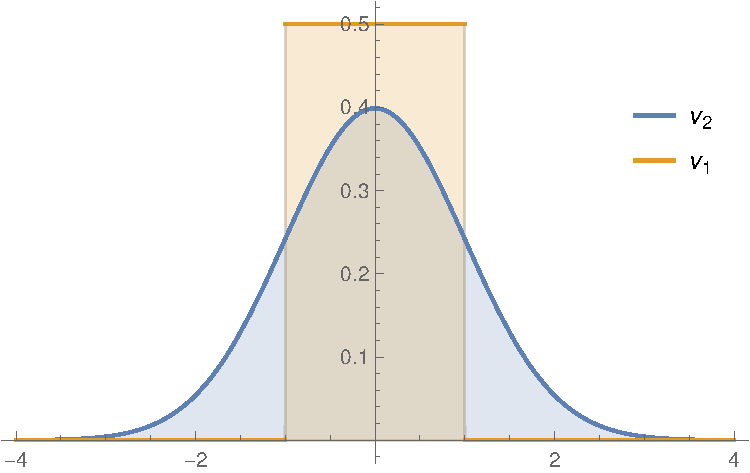
\includegraphics[height=.5\linewidth]{Chapters/OPT_line.pdf}
			\caption{Densities of $\nu_1$ and $\nu_2$}
		\end{minipage}
		\begin{minipage}{.49\textwidth}
			\centering
			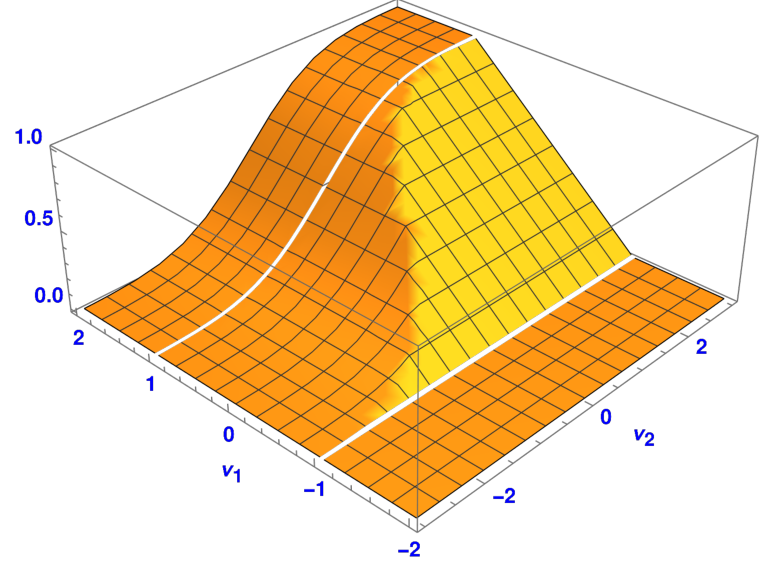
\includegraphics[height=.5\linewidth]{Chapters/cdf_line.pdf}
			\caption{CDF of optimal coupling}
		\end{minipage}
	\end{figure}
	We also draw the cumulative distribution function
	of optimal coupling between $\nu_1$ and $\nu_2$
	by \cite[Theorem 2.18]{villani2003topics}.
	% By McCann's displacement interpolation (\cite[Section 5.1.3]{villani2003topics}),
	% $\mu =[\frac{1}{2} \operatorname{Id} + \frac{1}{2} \nabla \psi]_{\#} \nu_1$ is the barycenter of $\mathbb{P}$.
	% Then the support of $\mu$ could not be compact,
	% otherwise the image of transport map is contained
	% in a compact set for $\nu_1$ almost everywhere.
\end{rmk}
